
\documentclass[letterpaper, 10 pt, conference]{ieeeconf}
\usepackage{graphicx}
\overrideIEEEmargins

\usepackage[utf8]{inputenc}
\usepackage[T1]{fontenc}
\usepackage{graphics}
\usepackage{amsmath}
\usepackage{amssymb}
\usepackage{booktabs}

\usepackage[hyphens]{url}
\usepackage{etoolbox}
\makeatletter
\def\fnum@table{TABLA~\thetable}
\patchcmd{\thebibliography}{\section*{References}}{\section*{Referencias}}{}{}
\patchcmd{\thebibliography}{{References}}{{Referencias}}{}{}
\makeatother
\renewcommand{\topfraction}{0.9}
\renewcommand{\dbltopfraction}{0.9}
\renewcommand{\textfraction}{0.07}
\renewcommand{\floatpagefraction}{0.85}
\renewcommand{\dblfloatpagefraction}{0.85}
\setcounter{topnumber}{3}
\setcounter{dbltopnumber}{3}

\title{\LARGE \bf
Clasificación de sonidos ambientales de ESC-50 mediante \textit{fine-tuning} del Audio Spectrogram Transformer
}

\author{Miguel Muñoz, David Cardenas y Mario Celis\\
Técnicas de Deep Learning (MAIA-4213), Universidad de los Andes}

\begin{document}

\maketitle
\thispagestyle{empty}
\pagestyle{empty}

%%%%%%%%%%%%%%%%%%%%%%%%%%%%%%%%%%%%%%%%%%%%%%%%%%%%%%%%%%%%%%%%%%%%%%%%%%%%%%%%
\section{Introducción}
Reconocer sonidos ambientales permite monitorear fauna con sensores acústicos pasivos, vigilar el ruido urbano y crear sistemas sensibles al contexto. Es difícil porque un mismo evento varía en duración y ruido de fondo, fuentes distintas (viento y olas) producen espectros parecidos y hay pocos datos etiquetados para entrenar redes profundas desde cero.

Este trabajo clasifica cada clip de 5\,s de ESC-50~\cite{piczak} en una de 50 clases agrupadas en 5 categorías. Los transformers~\cite{vaswani} relacionan todos los elementos de una secuencia mediante auto-atención; el Vision Transformer~\cite{vit} los aplicó a parches de imágenes, y el Audio Spectrogram Transformer (AST)~\cite{ast}, a espectrogramas log-mel. Preentrenado en AudioSet~\cite{audioset}, AST alcanza 95,6\,\% de exactitud en ESC-50 (5 folds)~\cite{ast}, lo que muestra el valor de transferir representaciones de un corpus grande a uno pequeño.

El objetivo es hacer \textit{fine-tuning} de AST durante 2 épocas y evaluar su precisión, recall y F1, identificando en qué clases falla y por qué. Se diseña un pipeline de espectrogramas para clips de 5\,s, se compara con una línea base MFCC y con AST sin entrenar, y se evalúan por ablación tres cambios: cabeza inicializada desde AudioSet, tasas por capa y SpecAugment~\cite{specaugment}. El modelo final, un ensamble de 3 semillas, obtiene F1-macro de 0,945 y exactitud de 0,948 en prueba.

\begin{figure*}[t]
    \centering
    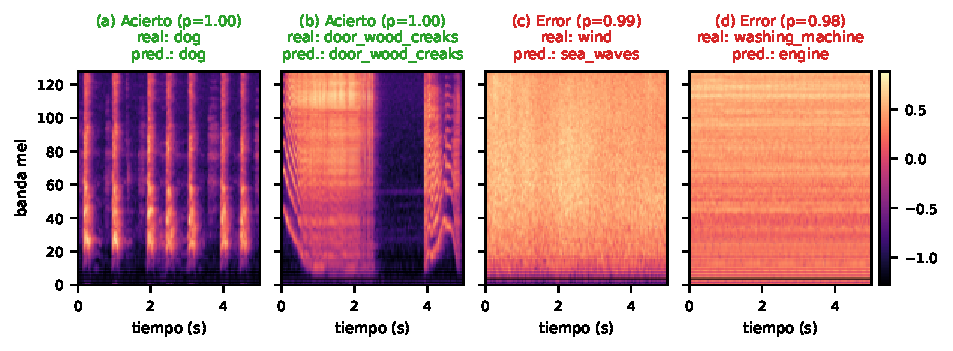
\includegraphics[width=\textwidth]{figs/v2_fig4_aciertos_errores.pdf}
    \vspace{-6mm}
    \caption{Espectrogramas log-mel normalizados de clips de prueba con la probabilidad que asigna el ensamble. (a, b) Aciertos de mayor confianza en dos categorías distintas. (c, d) Los dos errores de mayor confianza. La barra indica el valor log-mel normalizado.}
    \label{fig:cualitativo}
\end{figure*}

\section{Metodología}
\textbf{Datos.} ESC-50 tiene 2\,000 clips de 5\,s a 44,1\,kHz (40 por clase) en 5 folds~\cite{piczak}; se usó su versión en Hugging Face~\cite{hfdata}. Del fold~1, los 400 clips de prueba se reservaron para el reporte final, y los 1\,600 restantes se dividieron en 1\,279 de entrenamiento y 321 de validación (estratificando por clase y agrupando por grabación de origen para evitar fuga), con la que se tomaron todas las decisiones. Cada clip se pasa a mono a 16\,kHz y a un banco de filtros log-mel de 128 bandas (ventanas de 25\,ms cada 10\,ms), normalizado con las estadísticas de AudioSet para conservar la distribución del preentrenamiento. La entrada se fija en 512 tramas (5,12\,s), como hace AST para ESC-50~\cite{ast}; con las 1\,024 originales, la mitad sería relleno.

\textbf{Arquitectura y entrenamiento.} Se usa \url{MIT/ast-finetuned-audioset-10-10-0.4593}~\cite{ast} (86\,M de parámetros): $12\times50=600$ parches de $16\times16$ con paso 10, tokens [CLS] y de destilación~\cite{deit} y 12 bloques transformer de 12 cabezas. Las posiciones preentrenadas ($12\times101$) se adaptan con su recorte central de 50 posiciones de tiempo~\cite{ast}, y una cabeza nueva (LayerNorm y densa $768\rightarrow50$) reemplaza a la de AudioSet. Como cada clip tiene una sola clase, la salida es una softmax y se minimiza la entropía cruzada categórica, que maximiza la verosimilitud de esa distribución y penaliza los errores confiados~\cite{goodfellow}. Se usa AdamW~\cite{adamw} con tasa de $3\cdot10^{-5}$ en el transformer, para no destruir lo aprendido en AudioSet, y de $10^{-3}$ en la cabeza, que parte de cero; \textit{weight decay} de 0,01, \textit{warmup} del 10\,\%, \textit{clipping} con norma~1, lote efectivo de 16 ($8\times2$ por acumulación) y las 2 épocas del enunciado (160 pasos) (3\,min por época en un M2 Pro).

\textbf{Experimentos y métricas.} Se evaluó AST sin entrenar (\textit{zero-shot}), con la cabeza formada por las salidas de AudioSet equivalentes a cada clase (48 de 50). La ablación agrega a la receta base (A) un cambio por paso, conservado solo si sube el F1-macro de validación: (B) cabeza inicializada desde AudioSet; (C) tasas decrecientes por capa (LLRD)~\cite{ulmfit}, con $10^{-4}$ en la última capa, para que las capas altas se adapten más rápido que en A, y factor 0,75 por capa, dentro del rango que usa BEiT~\cite{beit}; y (D) SpecAugment~\cite{specaugment} con la configuración de AST para ESC-50 (máscaras de hasta 24 bandas y 96 tramas). La receta elegida se entrenó con 3 semillas (42, 7 y 123), promediadas en un ensamble~\cite{ensembles}; la línea base usa MFCC~\cite{mfcc} y regresión logística. Como las clases están balanceadas, se reportan exactitud y precisión, recall y F1 \textit{macro} (promedio sin ponderar de las 50 clases), por categoría y con intervalos de confianza del 95\,\% (IC) por \textit{bootstrap}.

\section{Resultados}






\textbf{Resultados cualitativos.} La Fig.~\ref{fig:cualitativo} muestra los dos aciertos y los dos errores de mayor confianza del ensamble. Los aciertos tienen una estructura temporal clara: el ladrido (a) es una serie de pulsos de banda ancha, y el crujido de la puerta (b) deja trazas tonales con barridos de frecuencia. Los errores son espectros casi estacionarios: el viento (c) cubre todas las bandas de forma uniforme, igual que las olas que predice el modelo, y la lavadora (d) muestra líneas horizontales constantes, como los armónicos de un motor, la clase predicha. En ambos el modelo se equivoca con probabilidad $\geq0{,}98$: falla en sonidos sin rasgos temporales distintivos, mientras que los animales, con armónicos y ritmos propios, no tienen errores.

\begin{table}[!t]
\centering
\caption{Val.: F1-macro en validación; demás columnas: métricas macro en prueba. A--D: pasos de la ablación (Sec.~II); LLRD: tasas por capa. Semillas: media $\pm$ desv. estándar de 3 entrenamientos de A.}
\label{tab:resultados}
\resizebox{\linewidth}{!}{
\begin{tabular}{lccccc}
\toprule
\textbf{Modelo} & \textbf{Val.} & \textbf{Exact.} & \textbf{Prec.} & \textbf{Recall} & \textbf{F1} \\
\midrule
MFCC + reg. logística & 0,459 & 0,435 & 0,455 & 0,435 & 0,427 \\
AST sin entrenar (\textit{zero-shot}) & 0,493 & 0,420 & 0,739 & 0,420 & 0,495 \\
\midrule
A: base (cabeza aleatoria) & \textbf{0,949} & 0,940 & 0,941 & 0,940 & 0,937 \\
B: A + cabeza AudioSet & 0,948 & 0,948 & 0,956 & 0,948 & 0,946 \\
C: A + LLRD & 0,905 & 0,895 & 0,905 & 0,895 & 0,892 \\
D: A + SpecAugment & 0,944 & 0,945 & 0,948 & 0,945 & 0,943 \\
\midrule
A, 3 semillas & -- & 0,938$\pm$0,008 & 0,941$\pm$0,008 & 0,938$\pm$0,008 & 0,935$\pm$0,010 \\
A, ensamble de 3 semillas & 0,948 & \textbf{0,948} & 0,951 & \textbf{0,948} & 0,945 \\
\bottomrule
\end{tabular}}
\end{table}

\begin{figure}[!t]
    \centering
    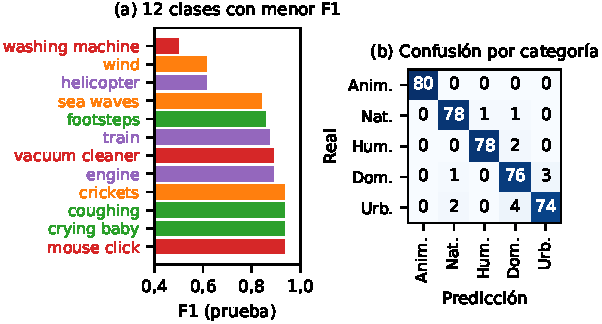
\includegraphics[width=\linewidth]{figs/v2_fig1_resultados.pdf}
    \vspace{-5mm}
    \caption{Ensamble final en prueba. (a) F1 de las 12 clases más difíciles; el color indica la categoría (azul: animales, naranja: naturales, verde: humanos, rojo: domésticos, morado: urbanos). Las 38 clases restantes tienen F1 $\geq$ 0,933. (b) Matriz de confusión por categoría, en número de clips.}
    \label{fig:resultados}
\end{figure}

\textbf{Resultados cuantitativos.} En la Tabla~\ref{tab:resultados}, AST sin entrenar ya supera a MFCC en prueba (F1 0,495 frente a 0,427). Ningún cambio superó a la receta base (A, 0,949 en validación), que fue la final: con 3 semillas logra $0{,}935\pm0{,}010$ en prueba, y el ensamble alcanza una exactitud de 0,948 y un F1 de 0,945 (IC: 0,917 a 0,962), 0,52 por encima de MFCC (IC: 0,48 a 0,58). Su mejora frente a la semilla 42 (+0,009) no es significativa (IC: $-0{,}005$ a $0{,}025$). Por categoría (Fig.~\ref{fig:resultados}b), el F1 va de 1,000 en animales a 0,933 en domésticos. De las 50 clases, 29 no tienen errores; las más difíciles son \textit{washing\_machine} (0,50), \textit{wind} y \textit{helicopter} (0,62) (Fig.~\ref{fig:resultados}a). De los 21 errores, 14 cruzan de categoría; los pares más confundidos son \textit{helicopter}$\rightarrow$\textit{washing\_machine} (4 clips), \textit{wind}$\rightarrow$\textit{sea\_waves} (3) y \textit{washing\_machine}$\rightarrow$\textit{engine} (2).

\section{Discusión}
El salto de F1 de 0,495 a 0,937 en solo 160 pasos confirma que el valor de AST está en la transferencia~\cite{ast}: los rasgos de AudioSet ya separan la mayoría de las clases y el ajuste solo los reorganiza. El \textit{zero-shot} tiene alta precisión (0,739) pero bajo recall (0,420) porque hereda los sesgos de AudioSet, que favorecen sus clases frecuentes; anularlos subió el F1 de validación de 0,446 a 0,493. La exactitud de 94,8\,\% queda cerca del 95,6\,\% reportado para AST~\cite{ast} con 5 folds y muchas más épocas, y supera la exactitud humana en ESC-50 (81,3\,\%)~\cite{piczak}. La brecha entre entrenamiento (0,994) y validación (0,950) indica un sobreajuste leve, esperable con 86\,M de parámetros y 1\,279 clips~\cite{goodfellow}.

Que ningún cambio ayudara se explica por lo corto del entrenamiento. La cabeza de AudioSet reduce la pérdida de la primera época de 1,18 a 0,46, pero la aleatoria la alcanza en la segunda; la diferencia en validación ($-0{,}001$) es menor que su ruido, y en prueba B fue mejor (0,946). Con LLRD, las capas bajas ($\sim\!4\cdot10^{-6}$) casi no se adaptan en 160 pasos y la tasa alta de arriba eleva la pérdida de validación (0,262 frente a 0,167): la adaptación gradual de~\cite{ulmfit} supone más épocas. SpecAugment bajó la exactitud de entrenamiento (0,994$\rightarrow$0,981) sin mejorar la validación: si el problema fuera la varianza, regularizar habría ayudado, así que con 2 épocas el límite es el sesgo~\cite{goodfellow}. Los 4 errores \textit{helicopter}$\rightarrow$\textit{washing\_machine} vienen de una sola grabación (\texttt{1-172649}), y \textit{washing\_machine} no tiene equivalente en AudioSet.

\textbf{Limitaciones y mejoras.} El F1 de validación seguía subiendo en la segunda época (de 0,907 a 0,949 en A), así que ningún modelo convergió: el tope de 2 épocas limita la comparación, sobre todo para LLRD y SpecAugment. Además, 321 clips de validación no distinguen diferencias menores a $\sim\!0{,}02$, y se usó un fold de los 5 del protocolo~\cite{piczak}. Se proponen validación cruzada, \textit{mixup}~\cite{mixup} y promediar recortes temporales~\cite{tta}.

\begin{thebibliography}{99}
\small
\bibitem{piczak} K. J. Piczak, ``ESC: Dataset for environmental sound classification,'' in \textit{Proc. 23rd ACM Int. Conf. Multimedia}, 2015, pp. 1015--1018.
\bibitem{vaswani} A. Vaswani \textit{et al.}, ``Attention is all you need,'' in \textit{Proc. Adv. Neural Inf. Process. Syst. (NeurIPS)}, 2017, pp. 5998--6008.
\bibitem{vit} A. Dosovitskiy \textit{et al.}, ``An image is worth 16x16 words: Transformers for image recognition at scale,'' in \textit{Proc. Int. Conf. Learn. Represent. (ICLR)}, 2021.
\bibitem{ast} Y. Gong, Y.-A. Chung, and J. Glass, ``AST: Audio spectrogram transformer,'' in \textit{Proc. Interspeech}, 2021, pp. 571--575.
\bibitem{audioset} J. F. Gemmeke \textit{et al.}, ``Audio Set: An ontology and human-labeled dataset for audio events,'' in \textit{Proc. IEEE Int. Conf. Acoust., Speech Signal Process. (ICASSP)}, 2017, pp. 776--780.
\bibitem{specaugment} D. S. Park \textit{et al.}, ``SpecAugment: A simple data augmentation method for automatic speech recognition,'' in \textit{Proc. Interspeech}, 2019, pp. 2613--2617.
\bibitem{hfdata} ConFit, ``ESC-50 demo (\texttt{confit/esc50-demo}),'' Hugging Face Datasets. [Online]. Available: \url{https://huggingface.co/datasets/confit/esc50-demo}
\bibitem{deit} H. Touvron \textit{et al.}, ``Training data-efficient image transformers \& distillation through attention,'' in \textit{Proc. Int. Conf. Mach. Learn. (ICML)}, 2021, pp. 10347--10357.
\bibitem{goodfellow} I. Goodfellow, Y. Bengio, and A. Courville, \textit{Deep Learning}. Cambridge, MA, USA: MIT Press, 2016.
\bibitem{adamw} I. Loshchilov and F. Hutter, ``Decoupled weight decay regularization,'' in \textit{Proc. Int. Conf. Learn. Represent. (ICLR)}, 2019.
\bibitem{ulmfit} J. Howard and S. Ruder, ``Universal language model fine-tuning for text classification,'' in \textit{Proc. 56th Annu. Meeting Assoc. Comput. Linguistics (ACL)}, 2018, pp. 328--339.
\bibitem{beit} H. Bao, L. Dong, S. Piao, and F. Wei, ``BEiT: BERT pre-training of image transformers,'' in \textit{Proc. Int. Conf. Learn. Represent. (ICLR)}, 2022.
\bibitem{ensembles} B. Lakshminarayanan, A. Pritzel, and C. Blundell, ``Simple and scalable predictive uncertainty estimation using deep ensembles,'' in \textit{Proc. Adv. Neural Inf. Process. Syst. (NeurIPS)}, 2017, pp. 6402--6413.
\bibitem{mfcc} S. Davis and P. Mermelstein, ``Comparison of parametric representations for monosyllabic word recognition in continuously spoken sentences,'' \textit{IEEE Trans. Acoust., Speech, Signal Process.}, vol. 28, no. 4, pp. 357--366, 1980.
\bibitem{mixup} H. Zhang, M. Cisse, Y. N. Dauphin, and D. Lopez-Paz, ``mixup: Beyond empirical risk minimization,'' in \textit{Proc. Int. Conf. Learn. Represent. (ICLR)}, 2018.
\bibitem{tta} K. Simonyan and A. Zisserman, ``Very deep convolutional networks for large-scale image recognition,'' in \textit{Proc. Int. Conf. Learn. Represent. (ICLR)}, 2015.
\end{thebibliography}

\end{document}
